\subsubsection{\stid{6.03} SNL ATDM Data and Visualization: IOSS and FAODEL} 

\paragraph{Overview} 
The SNL ATDM Data and Visualization project is developing data management software to improve how applications store and exchange large datasets efficiently on Exascale platforms. The data portion of this project is composed of two related efforts: (1) production work focused on improving Sandia's IOSS library for mesh datasets and (2) research work focused on developing new communication software named FAODEL that enables applications in a workflow to exchange data more efficiently.

\begin{description}
\item[IOSS:] IOSS is a production I/O library for mesh datasets used in many Sandia applications. IOSS provides a common front end for mesh data and supports multiple back-end file databases (e.g., Exodus and CGNS). This project is enhancing IOSS is two ways. First, a new hybrid mesh capability is being developed that will allow IOSS to support both structured and unstructured grids. This capability will allow users to use one API to access both forms of geometry data, thereby allowing them to more easily choose a meshing strategy that matches an application's needs. Second, IOSS is being enhanced to natively support Burst Buffers. These extensions will simplify the process of using Burst Buffers and accelerate general storage performance.


\item[FAODEL:] 
One of the challenges for production simulation work in Exascale computing is that workflows are becoming increasingly more sophisticated. Analysts routinely use workflows that use a variety of parallel tools to groom datasets, simulate different effects, and analyze a collection of results. Coupling different simulation tools together into a monolithic job is challenging due to library incompatibilities and fundamental differences in application runtimes (e.g., bulk synchronous parallel vs. asynchronous many-task (AMT) programming models). Many workflows instead run each parallel tool as an independent job and use the file system as the mechanism for handing off data in the workflow.

This project is developing new communication software called FAODEL (Flexible, Asynchronous, Object Data-Exchange Libraries) \footnote{In Gaelic, a \emph{faodhail} is a land bridge that forms between islands at low tide.} to provide better primitives for moving data between applications in Exascale platforms. In addition to supporting RDMA transfers of data from one MPI or AMT job to another, objects may be cached in distributed memory or nonvolatile memory resources.
\end{description}


\paragraph{Key  Challenges}
The key challenges for IOSS improvements are largely related to production stability. Adding support for hybrid meshes and Burst Buffers must be done in a way that does not cause significant changes to current APIs, while at the same time exposes enough functionality to be useful. \\

The key challenges in developing FAODEL to provide new data management services include the following:

\begin{enumerate}
  \item \textbf{Job-to-Job Support:} Workflows need a way to exchange data from one running application job to another in an efficient manner. While most RDMA communication libraries provide good \emph{intra-}job performance, they do not provide mechanisms to support \emph{inter-}job operations. Inter-job communication is complicated by the fact that the networks in many platforms have vendor-specific access controls that block inter-job communication by default. FAODEL must interface with these access controls. It must also avoid disturbing the application's native intra-job communication (e.g., MPI).
  \item \textbf{Flexible Management of Resources:} Service developers need a flexible way to reason about how an application's in-memory datasets are exposed to other applications. In addition to hosting data in dedicated staging nodes, applications should be able to host data in place for efficiency.
  \item \textbf{Asynchronous and Event-Driven Semantics:} AMT and analysis applications are asynchronous and require event-driven semantics that allow operations to trigger as objects migrate through the platform. Traditional remote procedure call (RPC) do not map well to this environment.
\end{enumerate}

\paragraph{Solution Strategy}
FAODEL is designed to provide communication libraries to implement advanced data management services. As illustrated in Figure~\ref{fig:faodel-diagram}(a), it is composed of five core libraries: a low-level RDMA portability library (NNTI), an out-of-band RESTful API for establishing job-to-job communication (Webhook), a network memory manager (Lunasa), an asynchronous communication engine (OpBox), and a distributed key/blob service (Kelpie). 

\begin{figure}[htb]
	\centering
	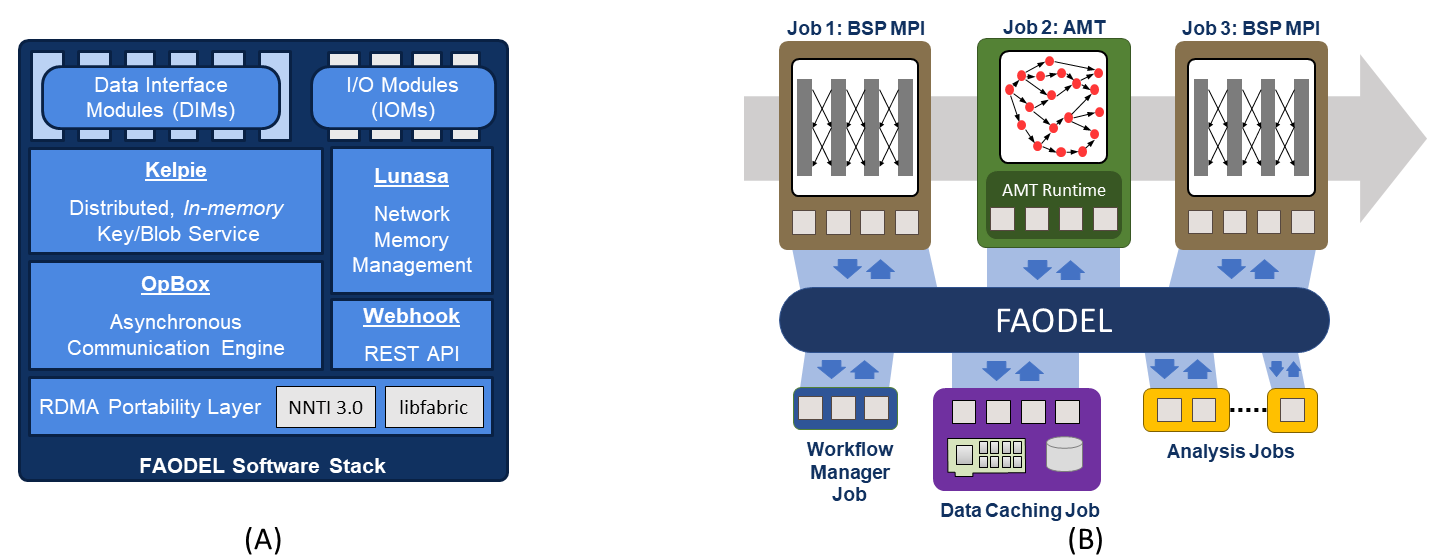
\includegraphics[width=6in]{projects/2.3.6-NNSA/2.3.6.03-SNL-ATDM/faodel-diagram}
	\caption{\label{fig:faodel-diagram}(a) FAODEL software stack and (b) a workflow example.}
\end{figure}


Figure~\ref{fig:faodel-diagram}(b) depicts an example of how multiple jobs of different types are connected together to implement a workflow. When a workflow manager dispatches these jobs to resources in the platform, it defines pools of nodes that are responsible for housing each dataset's objects. A pool may be internal or external to a job, and includes a definition of how data is distributed across pool members (e.g., a distributed hash table). Data transfers with a pool are coordinated through asynchronous communication state machines managed by OpBox. Downstream applications may choose to subscribe to data objects in a pool instead of polling for availability. If a requested object in a subscription is not available, OpBox pauses the request's state machine until it becomes available.

FAODEL users typically implement custom data interface modules (DIMs) to work with application-specific datasets. These interfaces decompose data into a collection of contiguous objects that can be dispersed to a pool as needed. While users are free to define how objects are structured and indexed in a DIM, the expectation is that data is organized in a form that is ready-to-use by applications. DIMs have been constructed for ATDM's EMPIRE and SPARC applications. A general mesh interface will be constructed to allow IOSS users to use FAODEL transparently.

\paragraph{Recent Progress}
\begin{enumerate}
  \item \textbf{FAODEL Integration into EMPIRE:} I/O interfaces have been constructed for EMPIRE/Fluid and EMPIRE/PIC to allow the applications to use FAODEL to store/retrieve mesh, field, and particle data. This implementation targets a checkpoint/restart use case but could be extended to couple EMPIRE to analysis tools.
  \item \textbf{Improved Asynchronous Messaging:} FAODEL allows users to express a series of communication operations as a state machine that is updated as relevant events happen. FAODEL was updated to allow different state machines to be processed in parallel to improve concurrency.
  \item \textbf{Initial Open Source Release:} FAODEL software was reviewed and approved for external release under the MIT license. The release is currently being transitioned to \url{https://github.com/faodel/faodel}.
\end{enumerate}


\paragraph{Next Steps}
\begin{enumerate}
  \item \textbf{EMPIRE/FAODEL Performance Experiments:} The FAODEL interfaces for EMPIRE will be tested and benchmarked on the Trinity platform. 
  \item \textbf{Transition to Sierra:} FAODEL will be updated to run on the CORAL/Sierra architecture.
\end{enumerate}
